% 卒業論文では英文アブストは必要ないので削除してください
\section*{Abstract}
This study proposes a method for detecting proximity droplet pairs by extracting local features in sparse droplet holograms instead of performing holographic reconstruction. First, the study formulates the local features on the spectral distribution of co-diameter proximity droplet holograms that have no depth direction distance. Then, the relationship between the geometric shape parameters of the local features and the distances between the droplets is illustrated. It is shown that proximity droplets can be detected by extracting local features on the spectral distribution. Second, a convolutional neural network-based image recognition model for detecting proximity droplet holograms is constructed using this property. Finally, the constructed model is used to perform inference on experimental data. Furthermore, the collision pair that led to coalescence is visualized using phase retrieval holography. It is shown that this method can be used to extract droplet collision and coalescence. If the method is further improved to achieve high-precision measurements, it will be possible to experimentally verify the collision efficiency in a turbulent field, thus contributing to the elucidation of cloud microphysical processes.
\newpage
\section*{概要}
本研究は,疎に分布する粒子ホログラムに対して像再生を行わず,局所特徴を抽出することで近接粒子組を検出する手法を提案する.はじめに,奥行方向距離を持たない同径近接粒子ホログラムのスペクトル分布上局所特徴を定式化し,局所特徴の幾何形状パラメータと粒子間距離の関係を示す.こうしてスペクトル分布上の局所特徴を抽出することで粒子近接を検出できることが示される.次に,この性質を用いて粒子ホログラムから近接検出を行う畳み込みニューラルネットワークベースの画像認識モデルを構築する.最後に,構築したモデルを用いて実験データに対する推論を行う.さらに,位相回復ホログラフィを用いて像再生し,併合に至った水滴組を可視化する.本手法によって水滴の衝突併合を抽出できることが示される.さらに手法の改善により高精度計測が可能になれば,乱流場における衝突効率を実験的に検証することで雲の微物理過程解明に寄与できる.

\newpage
\tableofcontents
\newpage
\pagenumbering{arabic} 
\section{緒言}
過去50年で気象災害の発生件数は5倍に増加し,気象災害による経済損失は世界全体で一日あたり3億8300万ドルに達する\cite{wmo2021}.損失や被害を最小化するためには国際的な減災対策が必要であり,その手段のひとつとして全球気候モデル\cite{climatemodel}や地球システムモデル\cite{earthsystem}による気候変動の将来予測が不可欠である.しかし,これらのモデルは一般に水平方向に\SI{100}{\km}ほどの格子解像度を有しており,雲内部の詳細な現象を計算し再現することは原理的に難しい\cite{grabowski2019}.雲粒の凝結や蒸発,衝突・併合による成長などといった,気候モデルの雲内部で再現できない微小スケールの物理現象を雲の微物理過程と呼ぶ.気候モデルにおいては雲の微物理過程の統計的な効果を経験的な近似手法であるバルク法で代替する\cite{kessler1969,lin1983,rutledge1984}.しかし,バルク法ではモデル全体の予測精度を向上させるために人為的なパラメータ調整が行われている\cite{hourdin2017}ため,線状降水帯などのメカニズムが未解明の降水現象や顕著気象に対する精度や信頼性の高い予測が困難である.したがって,気候モデルの精度・信頼性向上のために物理法則に基づく雲再現手法の開発が重要であり,そのために雲の微物理過程を解明することが課題である.

上記の課題解決のために,限定的な時空間領域における雲内部の現象を高い解像度で計算し再現する雲解像モデルを用いた研究が行われている\cite{khain2015,grabowski2019,morrison2020}.なかでも,確率的粒子法ベースの超水滴法\cite{shima2009,shima2020}は精度・性能ともに優れた雲解像モデルとして注目されている.超水滴法では,水滴・氷晶やエアロゾルなどの実粒子を,属性 $\bm{c}$ と多重度 $\xi$ を持つ仮想粒子である超水滴で代替する.属性 $\bm{c}$ は粒子の性質を,多重度 $\xi$ はその超水滴が表現する実粒子の個数を表す.超水滴同士の相互作用は確率モデルによって表現され,そのモンテカルロサンプリングによって時間発展を計算する.この手法は,雲の微物理過程を物理法則に基づいて解明するための有力な手段である.

超水滴法などの雲解像モデルで用いられる,水滴の併合による成長を記述する確率分布は,以下で与えられる\cite{gillespie1972,shima2020}.
\begin{equation}
    \label{intro:collisionprobability}
    P_{ij} = K(a_i, a_j) \frac{\mathrm{d}t}{\Delta V}
\end{equation}
$P_{ij}$は,領域$\Delta V$中にある半径 $a_i$ の水滴$i$と半径 $a_j$ の水滴$j$が,時間$\mathrm{d}t$の間に衝突・併合する確率を表す.$K(a_i,a_j)$は衝突併合カーネルと呼ばれ,系によっていくつかの表現があるものの,例えば無風状態で重力のみがはたらく理想的な状況では,以下のように与えられる\cite{pruppacher1996}.
\begin{equation}
    \label{intro:collisionkernel}
    % Pruppacker and Klett, Eq.(15-2)
    K(a_i, a_j) = E_{col}(a_i,a_j) \pi (a_i + a_j)^2 \left( U_{\infty,i} - U_{\infty,j} \right)
\end{equation}
ただし,$a_i>a_j$である.$U_{\infty}$は粒子の終端速度である.$E_{col}$は捕集効率(collection efficiency)と呼ばれ,水滴の水力学的相互作用を表す.半径が大きいコレクタ水滴の後流の影響で単純な剛体系として扱えないため重要である.捕集効率$E_{col}$は,さらに以下の衝突効率$E_{colli}$と併合効率$E_{coal}$に分解して表現できる.
\begin{equation}
    \label{intro:collectionefficiency}
    E_{col} = E_{colli} E_{coal}
\end{equation}
併合効率$E_{coal}$は,水滴組が衝突後併合へ至る割合で定義される.この系の衝突効率$E_{colli}$は,水滴$j$がコレクタ水滴$i$をかすめる水平オフセット$y_c$を用いて以下で定義される\cite{pruppacher1996}.
\begin{equation}
    \label{intro:collisionefficiency}
    E_{colli} = \frac{y_c}{\left( a_i + a_j \right) ^ 2}
\end{equation}
2つの水滴と$y_c$の関係をFig. \ref{fig:horizontaloffset}に示す.2つの水滴が十分な鉛直方向距離を持つとき,$y_c$はある値に収束し,小さな水滴$j$が$y_c$で定義する軌跡よりも内側にあれば,衝突が発生する.実際の$y_c$の値は理論的な解析や実験によって決定される.
\begin{figure}[b]
    \centering
    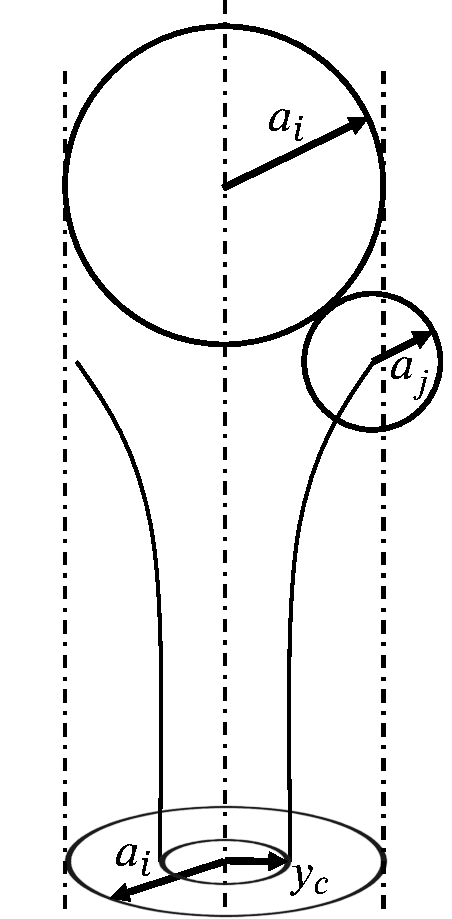
\includegraphics[width=0.4\linewidth]{./Figure/1_Introduction/yc.pdf}
    \caption{Schematic diagram of colliding droplet pair with horizontal offset for a grazing trajectory of the small droplet $y_c$; if the origin of the small droplet $j$ is inside the trajectory defined by $y_c$, the collision occurs.}
    \label{fig:horizontaloffset}
\end{figure}
無風状態や層流条件における衝突効率$E_{colli}$および併合効率$E_{coal}$の研究は2000年までにおおよそ完了しており,Pruppacher and Klett (1996)\cite{pruppacher1996}はその代表的な総説である.雲解像モデルにおける衝突併合モデルではDavis (1972)\cite{davis1972},Jonas (1972)\cite{jonas1972},Hall (1980)\cite{hall1980},Lin and Liu (1975)\cite{linliu1975}などの理論的な値を用いるか,Pinsky (2001)\cite{pinsky2001}の数値計算による導出が一般的である.超水滴法では前者の理論による値が用いられている.導出された分布は,風洞実験による結果との整合性が確認されている\cite{abbott1974, telford1955, woods1964}.

2000年頃から現在にかけては,実際の大気乱流条件におけるこれらの分布やその原理の解明が注目されている.乱流場における衝突・併合効率の研究は,主に層流条件における分布からの増加成分 $\Delta E$ について行われている.数値シミュレーションによる乱流場衝突効率の計算\cite{pinsky2008Part5},衝突効率の強化原理の説明\cite{pinsky2007Part4}などが行われ,実験では,風洞で生成した乱流場における衝突効率の測定値とその平均層流場との差が,乱流場における衝突効率の増加成分 $\Delta E_{colli}$ として報告されている\cite{vohl1999}.今後の乱流場における衝突・併合効率の研究で特に重要とされているのは,\SI{100}{\um}以上の水滴に対する衝突効率の評価と,水滴の分裂確率カーネルの導出である\cite{khain2018}.

以上より,筆者らの研究の最終的な目標は,乱流場における衝突・併合効率の実験的な検証および導出である.インラインホログラフィ\cite{gabor}を用いた3次元微粒子計測\cite{tanaka2016,kubonishi2018,nakatani2019}は,水滴の衝突・併合現象の直接的な観測に適している.また,GPUを用いた3次元像再生の高速化\cite{shimobaba2008, tanaka2019, nakai2022, tanaka2024}によって現実的な処理時間での計測が可能となった.これまで行われてきたホログラフィを用いた雲粒観測\cite{thompson1974,brown1989,fugal2009}では,雲粒の粒径分布や数密度などの統計量が得られているが,高速度撮影による衝突・併合現象の直接観測は行われていない.雲粒の高速度ホログラフィックイメージングは,雲粒の衝突・併合現象の直接観測とそれによる衝突・併合効率の評価を可能にする手法として期待される.

本研究では,高速度ホログラフィックイメージングによって水滴の衝突・併合効率の評価を行うために,ホログラフィを用いて水滴の衝突・併合現象を3次元観測するための手法の確立を目的とする.ホログラフィ計測でよく用いられる光波の逆伝搬による像再生は,GPUによって高速化されたもののその処理速度一枚あたり\SI{1.7}{s}ほどを要する\cite{nakai2022}.水滴の高速度撮影では\SI{4000}{fps}で撮影するため,衝突水滴を記録していないホログラムも含めてすべてのホログラムを像再生することは効率的ではない.したがって,はじめに本論文では,記録された粒子ホログラム画像から,ホログラム再生を行わず画像の局所特徴を直接抽出することで近接した粒子組を検出する手法を提案し,その原理を実験によって検証する\cite{nakai2023}.さらに,提案した原理を用いて設計した深層学習モデルによる画像認識を行い,実際に撮影した時系列水滴ホログラムから衝突水滴組を検出する.


本論文において,以降の各章で述べる内容を示す.第2章では,インラインホログラフィの原理,近接粒子ホログラムの理論,近接水滴抽出のための深層学習モデルの概要と,抽出したホログラムを像再生するために用いる位相回復ホログラフィの原理について説明する.第3章では,近接粒子ホログラムの局所特徴抽出のための検証実験,モデルの定義と学習方法,時系列水滴ホログラムの記録について述べる.第4章では,検証実験,モデルの学習,抽出結果の像再生それぞれについて結果を示し,考察を行う.第5章では,本論文の総括と結論を述べる.